\documentclass[a4paper,titlepage]{article}
\usepackage{fullpage}
\usepackage{graphicx}
\usepackage[compact]{titlesec}
\usepackage{enumitem}
\usepackage[pdftex]{hyperref}
\usepackage{subfigure}
\usepackage{float}
\setitemize{topsep=1pt,parsep=0.5pt,partopsep=1pt}
\title{Final project report:\\Machine Learning and Inductive Inference}
\author{Ingmar Dasseville \& Willem Van Onsem}
\date{December 23, 2011}
\hypersetup{pdfborder={0 0 0 0}}
\begin{document}
\begin{titlepage}
\maketitle
\end{titlepage}
\tableofcontents
\newpage
\section{Questions addressed by this research}
Most of the questions were already stated in the previous report together with the literature study. We will briefly repeat these questions together with additional questions we found while experimenting.
\begin{itemize}
 \item What are the categorization criteria in the context of strings and more specifically: to-dos.
 \item What algorithms can be used to link these criteria with affinity to certain tags. What is the performance of these algorithms.
 \item Why some algorithms perform better than others and if there is a difference between considering one label at a time or all of the labels at once.
 \item How to evaluate the system performance (quality of the predictions).
\end{itemize}
In the following sections we will describe different approaches to solve these problems, and the result of our experiments with regards to these questions.
\section{Categorization criteria}
We can classify a new cases on basis of the distance with other to-dos. Or we can obtain characteristics of the new to-do and classify samples based on the values of their characteristics.
\paragraph{}
Most of the characteristics are based on publications \cite{codeproject2,codeproject1} by Thanh Dao and \cite{Malakasiotis:2007:LTE:1654536.1654547} by P. Malakasiotis. We developed some criteria first and then saw them confirmed by these publications.
\subsection{Distance/Similarity measurements}
\label{ss:distanceStudy}
We did a study on distance metrics to find the most suitable methods. We studied the characteristics of different distance metrics with the given sample data. And analyzed the several distance metrics against the difference in tags. Therefore we used the $F$-measure metric on the tags. We made plots where the $x$-axis represents the $F$-measure of the tags of the samples. The $y$-axis represents the distance metric we want to test. We plotted every possible combination of two samples resulting in images on figure \ref{fig:metricStudy}. The color of a cell represents the percentage of cases in that column is at that distance.
\begin{figure}
\centering
\subfigure[Cosine Distance]{\includegraphics[width=0.47\textwidth]{CosineMetric.pdf}}
\subfigure[Dice Distance]{\includegraphics[width=0.47\textwidth]{DiceMetric.pdf}}
\subfigure[Euclidean Distance]{\includegraphics[width=0.47\textwidth]{EuclidDistance.pdf}}
\subfigure[Jacard Distance]{\includegraphics[width=0.47\textwidth]{JacardDistance.pdf}}
\subfigure[Levenshtein Word Distance]{\includegraphics[width=0.47\textwidth]{LevenshteinWordDistance.pdf}}
\caption{Study of several distance metrics.}
\label{fig:metricStudy}
\end{figure}

We strive to a plot where we see all the data is in the upper right triangle of the graph. That means that there are no to-dos who aren't related to another to-do, and have a low distance to each other\footnote{These points would be plotted in the lower left triangle.}. Having only a points on the diagonal would of course be ideal, however it is likely that for every combination of tags there are different to-do ``families'' that have the same affinity to the same tags, but are not related to each other. We modified similarity to distance by using $d=1-s$ with similarities who scale up to 1, or take the inverse. As we can see the cosine and dice metric perform quite well on this task. The word Levenshtein distance and the Jacard distance also has some correlation but also fill large parts of the lower left triangle. The word Levenshtein distance is a defined as the average of the minimal Levenshtein distance between each two words of the two to-dos.
\subsection{TeXHyphen}
A theory we developed ourselves is that the way words are spoken contains also information about the word. Therefore we implemented the TeXHyphen algorithm\cite[p.376-406]{knuth1986tex} of Donald E. Knuth. The idea is to split the word intro syllables and perform the Levenshtein Distance on the syllables of two words. This measurement wasn't successful partly because syllables with the same pronunciation are sometimes written differently, and partly because TeXHyphen made some errors. Later we found out the Soundex algorithm is also sometimes used as a similarity measurement. Due to lack of time, we didn't experiment with Soundex.
\subsection{Lucene.NET}
Lucene.NET is a framework that is used for search engines. It allows to tokenize characterstreams and can do basic token filtering, categorization and even spell checking. We used Lucene.NET to divide the to-dos intro a list of tokens and filter out irrelevant tokens like ``a'', ``the'' and ``will''. We also performed the ``Snowball English Stemming algorithm''\footnote{Also part of Lucene.NET} on those tokens, so that the meaning of those words became more clear. As a result we represented to-dos as a vector of stemmed words.
\subsection{WordNet.NET}
Another framework we experimented with was WordNet.NET. WordNet is a lexical database. WordNet uses ``synsets'' as the unit of textual information. This is a data structure including the word, a specific meaning and its synonyms. WordNet contains a database that represents an ``is-a'' hierarchy of synsets. The similarity between two words is defined as the length of the path to go from one synset to another in the hierarchy. WordNet contains a hierarchy for every type of word: verb, noun, adverb,... Troy Simpson and Thanh Dao published \cite{codeproject1} where they give a method to measure the similarity between two sentences. WordNet also allows the user to walk through the hierarchies. We used WordNet to generalize words so that for instance ``car'' and ``bicycle'' would be somehow related. This experiment however didn't improved system performance. This is probably caused by the grow of dimensionality of the problem when vectorizing the additional words.
\section{System outline}
\subsection{Votin gsystem}
We use a voting system as base for the tag system. With the voting system we are able to develop different approaches and test them independently, but combine them for a more accurate result. The voting system also is able to optimize certain operations. An important point of attention however is that all the taggers in the voting system, have the same interpretation of a value: all taggers return a number between 0 and 1
but a certain value must have the same level of certainty to all the taggers. Furthermore Weka supports a lot of binary classifiers who in most of the cases return only 0 or 1. This values give some taggers of the voting system a way to force their results through the voting system. Therefore these results are modified to 0.25 and 0.75.
\subsection{Classifiers via Mulan}

We ported the open-source java library Mulan\footnote{Mulan: A Java Library for Multi-Label Learning: \url{http://mulan.sourceforge.net/}} to C\# via IKVM\footnote{\url{http://www.ikvm.net/}}. Mulan is built on top op Weka with the purpose to extend Weka with possibilities for multi-label learning.
As in most literature there is a distinction between methods created specifically for multi-label learning and methods that convert the multi-label problem to multiple single-label problems.
After many experiments we decided to include two classifiers into our final program.
The first one we consider is the MLkNN algorithm. The second one Binary Relevance with an internal Naive Bayes.

\subsubsection{Mulan MLkNN}
\label{ss:mlknn}
MLkNN\footnote{Multi-Label k-Nearest Neighbours} is a natural extension to the k-Nearest Neighbours algorithm, known from single-label classification. Instead of just comparing the single class attributes from the unknown example to it's neighbours, it does this with all class tags.
As this algorithm uses the neighbours of a todo, we needed a distance metric to decide how we define ``closeness''.  as seen in \ref{ss:distanceStudy}. We ultimately decided to go with the cosine-metric, based on both taging-performance and runtime-performance.

\subsubsection{Mulan BR with NaiveBayes}
The other Recommender that is included in the final version of the project first transforms one problem with $n$ classes to $n$ problems with one class and then solves these individual, simpler problems with NaiveBayes. As NaiveBayes doesn't include support for String-attributes, the StringToWordVector-filter is applied to all instances (both training and test-data) before entering them in the classifiers. This filter includes converting lowercase and stemming.

\label{ss:sovectorclassif}
\subsection{ConcreteCustomVectorRecommender (J48 with our own vectorization)}
\label{ss:j48alg}
We used an alternative vector representation of every to-do before processing the data intro a Weka classifier. This vector was generated by \texttt{AbstractBasicTextVector}, every implementation of this class can choose how to modify a to-do intro a vector. We implemented \texttt{ConcreteBasicTextVector} with the Lucene.NET tokenizer, followed by custom classifiers. These additional classifiers were \texttt{Year}, \texttt{Month}, \texttt{Day}, \texttt{Number} and \texttt{Time} and were regular expressions or databases. It gives an interpretation to some data that is otherwise transformed into a huge collection af different tokens. The intention is to find these classifiers into the output of for example weka decision trees. Instead of using every possibly format of time into the tree of \texttt{\#appointment}, the tree would only contain \texttt{Time}. This would also result in parsing tokens the system hasn't seen before. We also used WordNet for these classifications. By adding all the synsets the system can find while moving up into the ``is-a'' hierarchy. This however resulted in bad performance. A possible explanation is that the classifiers generalize too much and because the number of attributes in the vector is approximately multiplied by four, what makes it difficult to see any rules in the vectors. If we had more time we thing adding more classifiers would increase the system performance.
\paragraph{}
After vectorizing the data as described above we used several classifiers of Weka. These classifiers could only classify a single tag at once. Each of these taggers was implemented in a subclass of \texttt{AbstractCustomVectorRecommender}. We used several techniques including decision trees, Bayesian networks and nearest neighbours. We finally used the J48 implementation of the C4.5 decision tree algorithm. Because of it's high precision en suitable recall.
\section{Evaluation of experiments}
All experiments were done by dividing the to-dos testcase into two partitions: one for training and one for testing. After training the system, the system was tested with both the training and testing data. Resulting into two result report: ``inner results'' were the results based on testing the training output. In theory one could get a 100\% correct result by caching all data. In most systems however we want to generalize the knowledge and avoid overfitting. The ``outer results'' are results based on the testing data, that means the system has never seen these to-dos before. The outer test actually tests if the system can generalize it's knowledge.
\paragraph{}
For all models we swept the percentage of testcases to be part of the trainingset from 2\% to 99\% with steps of 1\%. For each of these percentages, we simulated the model 10 times\footnote{Because most models learn slow, high amounts of testing isn't possible}. The result are datafiles containing for every simulation all evaluation metrics we will describe in subsection \ref{ss:evalmetrics}. Note that when the percentage reaches 99\%, the number of samples that belongs to the test dataset becomes small. As a result the results scatter, therefore we can't draw conclusions for these cases. However plotting these results shows how strong a model is on individual cases and gives us an impression about what happens when the percentage should go to 100\%, and be simulated on ``real'' new testcases.
\subsection{Evaluation metrics}
\label{ss:evalmetrics}
To evaluate the performance of our systems we used the following metrics: True-Positives (TP), False-Positives (FP), True-Negatives (TN), False-Negatives (FN), Precision, Recall, F-Measure, Accuracy and Hamming Loss. These metrics are well documented in \cite{Francis99performancemeasures} and generally used in machine learning and information retrieval. We need to make two notes on these metrics:
\begin{enumerate}
 \item The testcase is written by different people with each another way to tag items. So it's even difficult for a human to be consistent.
 \item The to-dos are evaluated by scores, we use the 50\% score as a hard line between tagging and not tagging. Therefore the metrics not always give a clear view.
\end{enumerate}
We also manually tested the systems with our own to-do list. To verify the system performance.

\subsection{Mulan MLkNN}
As we can see on figure \ref{fig:mlknnr} the perfomance of MLkNN is not very consistent. There is an increasing trend for both precision and recall. The precision varies between 50 and 80\%. But the recall doesn't get higher then 20\%. A possible reason for this is that our distance metric works very well for some cases but very bad for others. A more extensive comparison of the bad and good-performing test-sets would be necessary to improve the performance.

\begin{figure}
\centering
\subfigure[outer results]{\includegraphics[width=\textwidth]{MLkNNouter.pdf}}
\subfigure[inner results]{\includegraphics[width=\textwidth]{MLkNNinner.pdf}}
\caption{Results of the MLkNN.}
\label{fig:mlknnr}
\end{figure}

\subsection{Mulan BR with NaiveBayes}
As  we can see on figure \ref{fig:br} the performance of the BR algorithm is much more consistent than the MLkNN algorithm. The precision of the algorithm rises quickly as the testcases raises to 20\% of the size. And the recall keeps increasing as the number of testcases grows. In the end, both the precision and recall are about 55\%. This performance is far warse then MLkNN but as the recall is a lot better, the netto result is in favor of BR. We can see in the outer results that the dataset is very good at fitting small sets, this could be a sign of overfitting. Investigating how to counter this behavior would be the next step for increasing the performance in this metric.

\begin{figure}
\centering
\subfigure[outer results]{\includegraphics[width=\textwidth]{vectorClassifinner.pdf}}
\subfigure[inner results]{\includegraphics[width=\textwidth]{vectorClassifouter.pdf}}
\caption{Results of the Mulan BR with NaiveBayes.}
\label{fig:br}
\end{figure}

\subsection{ConcreteCustomVectorRecommender (J48 with our own vectorization)}
As we can see on figure \ref{fig:ccvrresults} the algorithm gives good inner results with a precision of 95\% and a recall, accuracy and F-measure of 60\%. These data converge also fast - around 20\% - and have very few outliers and a low variance. The hamming loss - about 7\% - also indicates that few of the models are in fact overgeneralizing the training data. The outer results are as often lower. The precision reaches about 80\% but recall accuracy and F-measure remain on 40\%. This indicates that the system in most cases will only apply a tag on the todo if it is quite sure. A problem that we have encountered many times with decision trees and classifiers in common. However finding a way to make the system more ``brave'' is not that trivial. Using ``fake'' training data could be a solution however experiments shown that that a higher recall is bought off by a much lower precision. The system converges at about 30\% and remains consistent until about 95\% meaning even on individual cases there are most of the times no real surprises. The range of each of the metrics is about 10\%, meaning of course that the algorithm is somewhat sensible to differences in the trainingset.
\begin{figure}
\centering
\subfigure[outer results]{\includegraphics[width=\textwidth]{j48outer.pdf}}
\subfigure[inner results]{\includegraphics[width=\textwidth]{j48inner.pdf}}
\caption{Results of the ConcreteCustomVectorRecommender.}
\label{fig:ccvrresults}
\end{figure}
\section{The theses-dataset}
As our application doesn't include hardcoded properties of the todo-dataset, we can use our application directly on other datasets for the multilabel-classification problem. We tested our application on the given theses-dataset. The Naive Bayes algorithm of section \ref{ss:sovectorclassif} didn't perform very well, it's precision plummeted to 5\%. On the other hand, the J48 of \ref{ss:j48alg} held it's cause and performed reasonably well with both precision and recall of more than 50\%. 
We assume that the Naive Bayes performs bad because the ratio of  the number test cases  and the number of tags and went down drastically. Apparently decision tree algorithms such as J48 don't suffer as much from these worse conditions. 

\section{The Server}
The web application communicates with an ASP.NET-server via AJAX. Every time a key is released in the input-box, the current contents of the text box are send to the server and tags are suggested. For every suggested tag there is a check-box which is checked by default. 
When the todo is entered in the system, every checked text box is added as a tag to the todo. The color of the text reflects the certainty the system assigns to the tag. The shade changes from red to green as the confidence increases. Under these check-boxes the request number is noted. Every time a (partial) todo is sent to the server this number is increased by one. This number is sent by the server, so it can be used visually ensure that the server has sent his reply.
\begin{figure} \centering 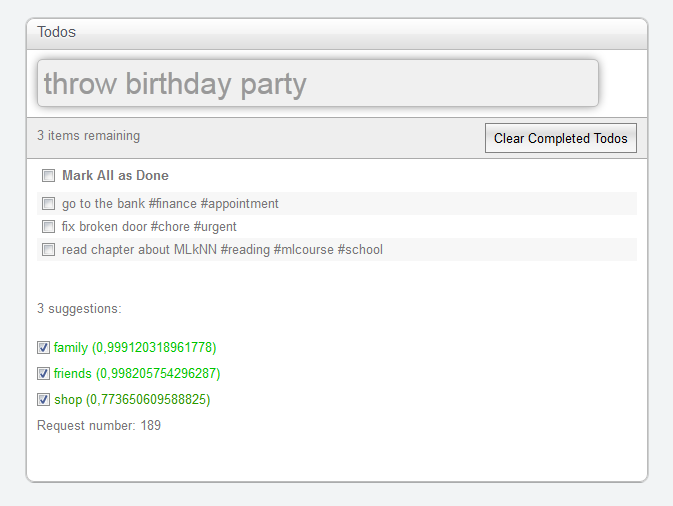
\includegraphics[width=0.70\textwidth]{screenshot.PNG} \caption{Our webapplication} \end{figure}
Inside the server, we use a Voting System as master-classifier. On the first-access of the page the classifiers are initialized and then queried via AJAX as explained before. 

When the server is running (the WebApp-project in Visual Studio), the application can be accessed by going to \url{http://urlFromServer/todos/index.aspx}. The first time this page is loaded on a server this can be very slow as the classifiers need a few seconds to initialize as the page is loaded.

\section{About the SproutCore framework}
Our experiences with the SproutCore framework are not very good. SproutCore looks like a good framework for the cases where no server is available, but when you try to couple it to a server everything becomes very complicated. We wanted to work in the .NET-framework so we imported the example project in a ASP.NET-server. ASP.NET is a type-safe language, so when you use an object as a target for by example Ajax-communication, he seeks for the corresponding id in the page. 
The problem is that SproutCore generates it's DOM dynamically so the ASP-code cannot be checked, so it won't compile. A few hacks, and even one little change in the SproutCore-framework source file was necessary to get everything to work. In the end, it would be have been simpler to write everything from scratch. 

\section{Time and project management}
The time estimates where quite realistic. Although we didn't think it would make much sense spending both much time with SproutCore as this part has no strong link with the course. Willem focused more on the theoretic part of the algorithms and Ingmar more on the integration of the todo-dataset in these algorithms. In the table you can see the division of the work expressed in hours.
\begin{table}[H]
\centering
\begin{tabular}{lcc}
&Ingmar&Willem \\
Literature Study & 11 & 14\\
SproutCore & 9 & 1\\
To-dos & 1 & 1\\
Machine Learning & 13 & 25\\
Todo-Application & 14 & 10 \\
Master theses & 8 & 4\\
Report & 5 & 7\\
\hline
Total & 61 & 62
\end{tabular}
\end{table}
\section{Conclusions}
\begin{itemize}
 \item There exists a lot of criteria for input, classification algorithms and evaluation metrics. Testing all of them is impossible, one can only make progress by developing a solution step by step. Our discussion on distance metrics showed us that analyzing the problem layer by layer is more effective.
 \item It takes a great effort to make classifiers generalize knowledge on a consistent way and make them ``brave'' enough to classify a sample with uncertainties.
 \item Doing all of the generalization yourself is not a good idea. The experiment with the WordNet library showed that by giving the system all possible generalizations, this could lead to overgeneralization resulting in low precision.
\end{itemize}
\nocite{*}
\bibliographystyle{plain}
\bibliography{bib}
More references are in the literature study submitted earlier.
\end{document}